\section{Definitions}
\label{sec:defs}
Following the definitions provided by Liffiton, et. al.~\cite{liffiton2016fast}, a constraint system $C$ is an ordered set of abstract constraints $\{C_1, C_2,\dots,C_n \}$ over some set of variables. Each constraint $C_i$ restricts the assignment of those variables in some way. For every subset $S \subseteq C$, we have a method of determining whether $S$ is \em{satisfiable} (\sat), meaning there exists an assignment that is allowed by all $C_i \in S$ or \em{unsatisfiable} (\unsat), meaning no such assignment exists. 

It is of interest to identify certain subsets of a constraint system that have particular properties. 

A minimal unsatisfiable subset (MUS) $M$ of a constraint system $C$ is a subset $M \subseteq C$ such that  $M$ is unsatisfiable and $\forall c \in M$, $M$\textbackslash $\{c\}$ is satisfiable. This is the minimal explanation of a constraint systems infeasability. 

A related subset of a constraint system is the minimal correction set (MCS) $M$ of a constraint system $C$ is a subset $M \subseteq C$ such that  $C$ \textbackslash $M$ is satisfiable and $\forall S \subset M$, $C$\textbackslash $S$ is unsatisfiable. In other words, the removal of the constraints in $M$ from $C$ ``corrects'' the infeasibility of $C$ and these are the minimal of such sets in $C$.

A duality exists between these two sets and it is defined in terms of {\em hitting sets}. A hitting set of a collection of sets $A$ is a set $H$ such that every set in $A$ is hit by $H$. That means that $H$ contains at least one element from every set in $A$. A {\em minimal hitting set} $H_{min}$ is a hitting set that is subset minimal, i.e. no element can be removed from $H_{min}$ without removing its hitting set property and missing some set in $A$. Every MUS of a constraint system is a minimal hitting set of the systems MCSs and every MCS is a minimal hitting set of its MUSs~\cite{reiter1987theory, de1987diagnosing, liffiton2016fast}. 



\begin{comment}
\subsection{Fault Tree Analysis} 
The use of fault trees are common in many safety assessment processes and the ability to generate the cut sets needed for the construction of the fault tree is a useful part of any safety analysis tool. The fault tree is a safety artifact commonly referenced in requirement protocol documents such as ARP4761, ARP4754, and AIR6110~\cite{SAE:ARP4761,SAE:ARP4754A,AIR6110}.

% There are two main types of fault tree analysis that we differentiate here as \textit{qualitative} analysis and \textit{quantitative} analysis. In qualitative analysis, the structure of the fault tree is considered and the cut sets are a way to indicate which combinations of component failures will cause the system to fail. On the other hand, in quantitative analysis the probability of the TLE is calculated given the probability of occurance of the basic events. By being able to generate cut sets based on both probability and cardinality, this allows for either form of FTA to be created. 

A Fault Tree (FT) is a directed acyclic graph whose leaves model component failures and whose gates model failure propagation~\cite{0f356f05e72f43018211b36f97c8854a}. The system failure under examination is the root of the tree and is called the Top Level Event (TLE). The node types in a fault tree are \textit{events} and \textit{gates}. An event is an occurrence within the system, typically the failure of a subsystem down to an individual component. Events can be grouped into Basic Events (BEs), which occur independently, and \textit{intermediate events} which occur dependently and are caused by one or more other events~\cite{historyFTA}.  These events model the failure of the system (or subsystem) under consideration. The gates represent how failures propagate through the system and how failures in subsystems can cause system wide failures. The two main logic symbols used are the Boolean logic AND-gates and OR-gates. An AND-gate is used when the undesired top level event can only occur when all the lower conditions are true. The OR-gate is used when the undesired event can occur if any one or more of the next lower conditions is true. This is not a comprehensive list of gate types, but we focus our attention on these two common gate types. 
\begin{figure}[h]
\begin{center}
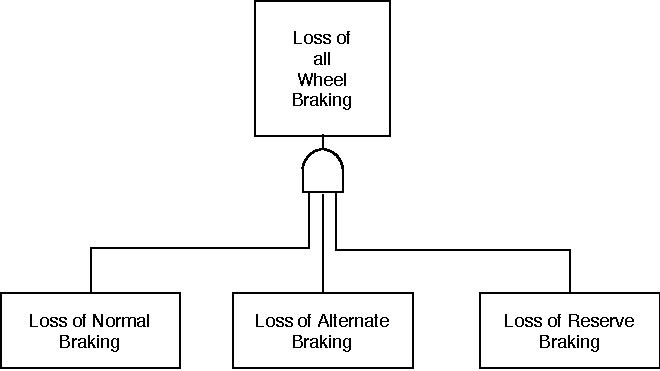
\includegraphics[width=8cm]{images/introFT2.pdf}
\caption{A simple fault tree} \label{fig:introFT}
\end{center}
\end{figure}

Figure~\ref{fig:introFT} shows a simple example of a fault tree based on SAE ARP4761~\cite{SAE:ARP4761}. In this example, the top level event corresponds to an aircraft losing all wheel braking. In order for this event to occur, all of the basic events must occur. This is seen through the use of the AND gate below the top level event. The gates in the fault tree describe how failures propagate through the system. Each gate has one output and one or more inputs. In Figure~\ref{fig:introFT}, the AND gate has three inputs and one output. The leaves of the tree represent the basic events of the system. %and 
In the case of this fault tree, these three events are also the Minimal Cut Sets (MinCutSets) for this top level event. A MinCutSet is the minimal set of basic events that must occur together in order to cause the TLE to occur. Generating and analyzing these MinCutSets is important to FTA and has been an active area of interest in the research community since fault trees were first described in Bell Labs in 1961~\cite{historyFTA,0f356f05e72f43018211b36f97c8854a}. 

There are two main types of fault tree analysis that we differentiate here as \textit{qualitative} analysis and \textit{quantitative} analysis. In qualitative analysis, the structure of the fault tree is considered and the MinCutSets are a way to indicate which combinations of component failures will cause the system to fail. On the other hand, in quantitative analysis the probability of the TLE is calculated given the probability of occurrence of the basic events. By being able to generate MinCutSets
based on both cardinality and probability, this allows for either form of FTA to be created. 



\end{comment}




